\documentclass[UTF8,a4paper,12pt]{ctexart}
\usepackage{amsmath,amssymb}
\usepackage{graphicx}
\usepackage{booktabs}
\usepackage{fvextra}
\usepackage{float}
\usepackage{placeins}
\usepackage{needspace}
\usepackage{geometry}
\usepackage{hyperref}
\geometry{left=2.5cm,right=2.5cm,top=2.5cm,bottom=2.5cm}
\hypersetup{colorlinks=true,linkcolor=blue,urlcolor=blue}

\title{基于几何光学的教室黑板镜面反射模型\\与有限俯仰角下的最优调节方案}
\author{王瑞德\quad 王家件\quad 胡益玮\\广东省广州市广州大学附属中学\\高二\quad 指导老师：沈云}
\date{2026年4月}

\begin{document}
\maketitle

\begin{abstract}
教室黑板与一体机屏幕在强光下易产生镜面反射，导致局部座位看不清板书。本文在单侧窗户平行光入射、黑板可绕底边小角度俯仰的设定下，先建立竖直截面内的反射模型，再在此基础上将座位区抽象为水平面上的长方形区域，用离散网格判定「反射光与视线是否共线（在阈值角内）」以刻画受害范围。对每个授课时刻，在最大俯仰角不超过 $\theta_{\max}$ 的硬约束下，用一维扫描求使前排代表座位消除眩光的\textbf{最小必要}俯仰角 $\theta^\ast(t)$。数值仿真表明：在示意参数下，早读后段（如 $8{:}00$）受害座位面积比例可由约 $11.6\%$ 降至约 $4.3\%$，并给出可调铰链与限位角的改造建议。

\textbf{关键词：}镜面反射；黑板俯仰；眩光；离散优化；教室采光
\end{abstract}

\section{问题重述}
日常教学中，前排同学常因黑板局部反光看不清板书，一体机玻璃屏尤为明显。光源主要为日光与灯光的镜面反射。拉窗帘、调座位、换哑光板各有代价。更根本的做法是\textbf{略微改变黑板法向}，使反射光偏离学生视域。本题要求：建立几何光学模型，求\textbf{有限转角}下的最优（本文取「最小必要」）俯仰方案，并给出可落地改造思路。

\section{模型假设}
\begin{enumerate}
  \item 以\textbf{平行光}近似太阳光；主光源从教室\textbf{单侧窗户}入射，方向随时间缓慢变化。
  \item 黑板（含一体机显示区中的镜面分量）抽象为\textbf{平面镜面}，绕与黑板底边重合的水平轴俯仰，整板同角 $\theta$。
  \item 座位区在水平面内为\textbf{长方形}；学生眼高取统一值 $h_e$（坐姿统计均值）。
  \item 当黑板某采样点处反射光方向与「该生看向该点」的视线夹角小于阈值 $\varepsilon$ 时，判为\textbf{受害}（眩光显著影响辨认）。
  \item 忽略多次反射与散射的次要贡献；不讨论偏振与色散。
\end{enumerate}

\section{符号说明}
\begin{table}[htbp]
\centering
\begin{tabular}{@{}ll@{}}
\toprule
符号 & 含义 \\
\midrule
$\theta$ & 黑板俯仰角（相对竖直位置，单位 $^\circ$） \\
$\theta_{\max}$ & 允许的最大俯仰角（书写与观看约束） \\
$\theta^\ast(t)$ & 时刻 $t$ 的最小必要俯仰角 \\
$\mathbf{n}$ & 黑板外法向（指向教室一侧） \\
$\mathbf{l}$ & 入射光方向（指向板面，满足 $\mathbf{l}\cdot\mathbf{n}<0$） \\
$\mathbf{r}$ & 反射光方向（自板面射出） \\
$\varepsilon$ & 眩光判定半角阈值 \\
\bottomrule
\end{tabular}
\end{table}

\section{模型建立}

\subsection{反射定律（向量形式）}
设 $\mathbf{l}$、$\mathbf{n}$ 均为单位向量，$\mathbf{n}$ 为外法向。反射方向
\begin{equation}
  \mathbf{r}=\mathbf{l}-2(\mathbf{l}\cdot\mathbf{n})\mathbf{n}.
\end{equation}

\subsection{竖直截面几何（板书推导主模型）}
取含黑板法向与窗户主入射方向的\textbf{竖直平面}。黑板底边离地 $z_{\mathrm{bot}}$，板高 $H$，俯仰后板面法向随 $\theta$ 变化。太阳方向在该平面内（或由三维方向投影）记为随时间变化的入射单位向量。

\subsection{长方形教室与座位受害判定（俯视展示）}
建立右手系：$X$ 轴垂直黑板指向教室内侧，$Y$ 轴沿黑板宽度方向，$Z$ 轴竖直向上。黑板底边过点 $(0,y_{\min},z_{\mathrm{bot}})$，板面离散为 $n_u\times n_v$ 个采样点 $\{P_k\}$。座位平面 $z=h_e$，在 $[x_{\min},x_{\max}]\times[y_{\min},y_{\max}]$ 上网格化，网格中心为眼睛位置 $E_{ij}$。

对固定 $(\theta,t)$，取该时刻入射方向 $\mathbf{l}(t)$。若存在某 $P_k$ 使
\begin{equation}
  \angle\big(\mathbf{r}_k,\ \overrightarrow{P_kE_{ij}}\big)<\varepsilon,\qquad
  \mathbf{r}_k=\mathbf{l}-2(\mathbf{l}\cdot\mathbf{n})\mathbf{n},
\end{equation}
则座位 $(i,j)$ 判为受害。

\subsection{逐时刻优化（最小必要角）}
对前排\textbf{代表座位} $E_0$（本文取近第一排、$y=0$ 处），离散扫描 $\theta\in[0,\theta_{\max}]$（步长如 $0.05^\circ$），取\textbf{第一个}使 $E_0$ 不受害的 $\theta$ 作为 $\theta^\ast(t)$，体现「尽量少动黑板」。若全程受害，则取 $\theta_{\max}$ 并标记为不可行（可配合窗帘等辅助措施）。

\section{模型求解与算法}
\begin{enumerate}
  \item 输入教室与黑板几何、$\varepsilon$、$\theta_{\max}$、时间离散 $\{t_m\}$。几何与采光参数参照《建筑采光设计标准》普通教室的推荐层高与采光要求选取，使典型教室尺寸与日照条件具有工程意义。
  \item 对每个 $t_m$，生成 $\mathbf{l}(t_m)$（本文用水平方位角随授课时段线性扫过、仰角缓变的示意函数模拟广州地区晴天侧窗工况）。
  \item 一维扫描得 $\theta^\ast(t_m)$。
  \item 对选定时刻，计算 $\theta=0$ 与 $\theta=\theta^\ast$ 下座位网格受害二值图，输出面积比例 $\rho_0,\rho_\ast$。
\end{enumerate}

程序使用 Python（NumPy/Matplotlib）实现。为便于评委和读者理解数值实现，下面给出反射与眩光判定的关键程序片段。

\Needspace{16\baselineskip}
\subsection*{输入数据与参数设置}
\begin{table}[H]
\centering
\begin{tabular}{@{}lll@{}}
\toprule
类别 & 参数 & 取值（示意） \\
\midrule
黑板几何 & 底边离地 $z_{\mathrm{bot}}$ & $1.0\,\mathrm{m}$ \\
黑板几何 & 板高 $H$ & $1.2\,\mathrm{m}$ \\
黑板几何 & 板宽方向范围 $y\in[y_{\min},y_{\max}]$ & $[-2.0,\,2.0]\,\mathrm{m}$ \\
座位区域 & 深度范围 $x\in[x_{\min},x_{\max}]$ & $[2.0,\,8.0]\,\mathrm{m}$ \\
座位区域 & 宽度范围 $y\in[y_{\min},y_{\max}]$ & $[-2.5,\,2.5]\,\mathrm{m}$ \\
座位区域 & 眼高 $h_e$ & $1.15\,\mathrm{m}$ \\
光学判据 & 眩光阈值角 $\varepsilon$ & $9^\circ$ \\
控制约束 & 最大俯仰角 $\theta_{\max}$ & $8^\circ$ \\
离散设置 & 黑板采样点数 $n_u\times n_v$ & $8\times6$ \\
离散设置 & 座位网格数 $n_x\times n_y$ & $28\times24$ \\
时间离散 & 授课时段与步长 & $8{:}00$--$17{:}00$, $\Delta t=0.5\,\mathrm{h}$ \\
\bottomrule
\end{tabular}
\caption{仿真输入数据与参数设置}
\label{tab:input}
\end{table}

\Needspace{14\baselineskip}
\subsection*{关键程序片段（Python）}

\fvset{fontsize=\scriptsize}
\begin{Verbatim}[breaklines=true,breakanywhere=true,frame=single]
def reflect(incident_to_surface: np.ndarray, n_out: np.ndarray) -> np.ndarray:
    """入射方向指向板面，外法向 n_out 指向教室（+X 侧）；满足 dot(l,n_out)<0。"""
    l = incident_to_surface / np.linalg.norm(incident_to_surface)
    r = l - 2.0 * np.dot(l, n_out) * n_out
    return r / np.linalg.norm(r)


def seat_glare(eye: np.ndarray, theta_deg: float, l_in: np.ndarray) -> bool:
    pts, n = sample_board_points(theta_deg)
    eps = np.radians(P.epsilon_deg)
    if np.dot(l_in, n) >= 0:
        return False
    for p in pts:
        r = reflect(l_in, n)
        w = eye - p
        wn = np.linalg.norm(w)
        if wn < 1e-6:
            continue
        v = w / wn
        c = float(np.clip(np.dot(r, v), -1.0, 1.0))
        if float(np.arccos(c)) < eps:
            return True
    return False
\end{Verbatim}
\FloatBarrier

\section{结果与分析}

\subsection{逐时刻最小必要俯仰角}
图 \ref{fig:theta} 给出 $8{:}00$--$17{:}00$、步长 $0.5\,\mathrm{h}$ 的 $\theta^\ast(t)$。可见在示意入射角设定下，清晨若干时刻需要 $1^\circ$--$3^\circ$ 量级的调节，其余时段可与竖直位置接近。

\begin{figure}[htbp]
  \centering
  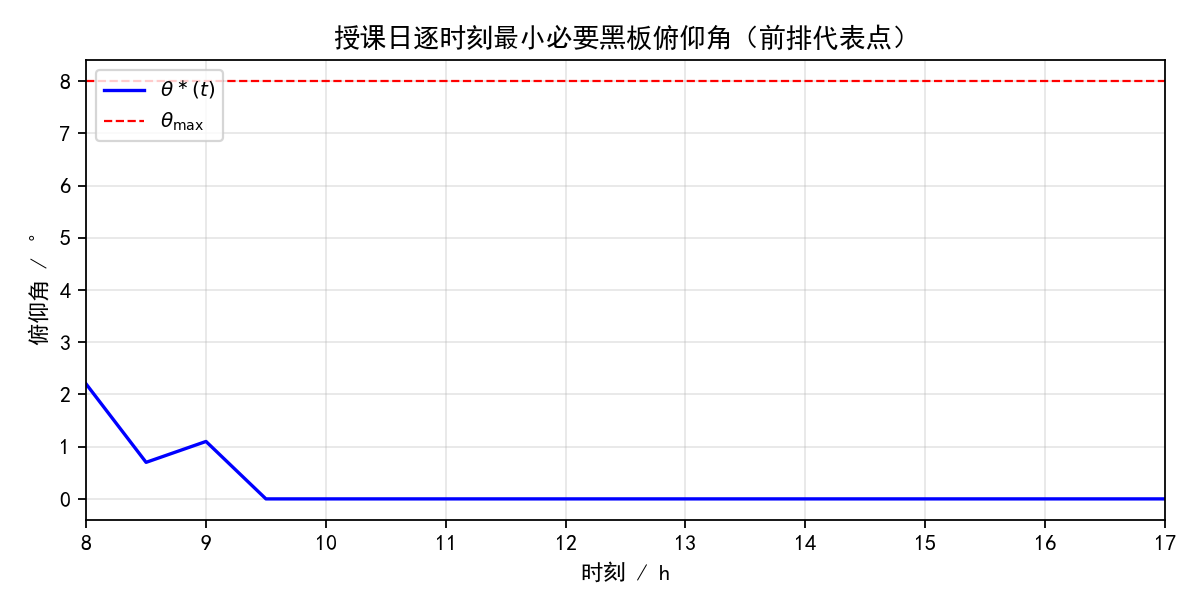
\includegraphics[width=0.92\linewidth]{figures/theta_of_t.png}
  \caption{授课日逐时刻最小必要黑板俯仰角（前排代表点）与 $\theta_{\max}$ 上界示意}
  \label{fig:theta}
\end{figure}
\begin{figure}[htbp]
  \centering
  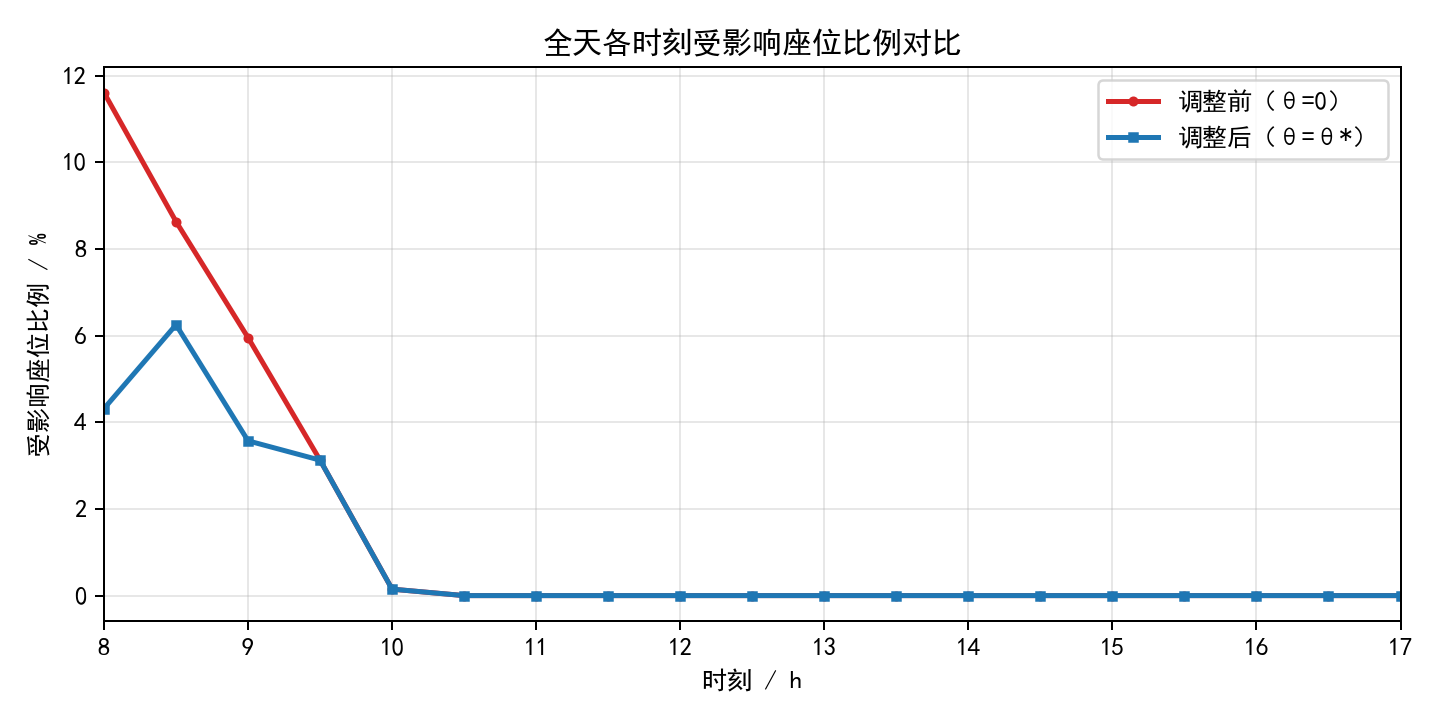
\includegraphics[width=0.92\linewidth]{figures/affected_ratio_compare.png}
  \caption{全天各时刻受影响座位比例对比：调整前（$\theta=0$）与调整后（$\theta=\theta^\ast$）}
  \label{fig:ratio}
\end{figure}
\FloatBarrier
\FloatBarrier

\subsection{受害座位区域：调节前后对比（长方形教室）}
在\textbf{同一时刻、同一太阳方向}下，图 \ref{fig:top8} 对比 $\theta=0$ 与 $\theta=\theta^\ast$ 的俯视填色图（红色表示该格中心座位受害）。数值上，本组示意参数在 $t=8{:}00$ 时，受害格点比例由约 $11.6\%$ 降至约 $4.3\%$。

\begin{figure}[htbp]
  \centering
  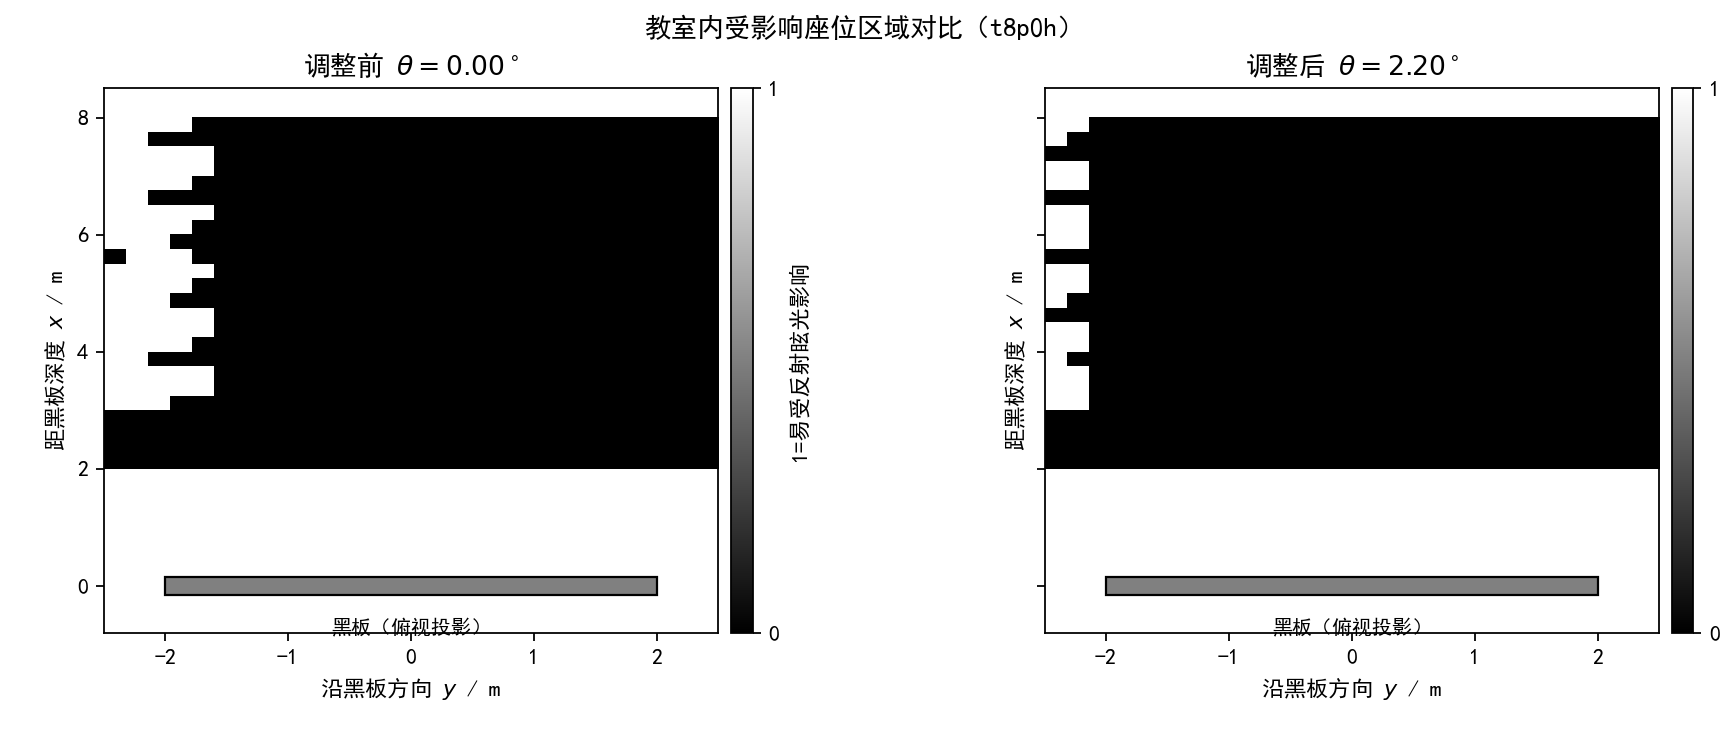
\includegraphics[width=\linewidth]{figures/topdown_compare_t8p0h.png}
  \caption{$t=8{:}00$ 示意：调节前后受害座位区域对比（俯视）}
  \label{fig:top8}
\end{figure}
\FloatBarrier

此外，程序自动搜索「在原始布置下存在眩光、且可通过旋转使全教室受害比例降为 0」的代表性时刻。根据本次仿真，代表时刻为 $t=9{:}30$，对应无眩光旋转角约 $\theta=1.65^\circ$。图 \ref{fig:topnog} 给出了该时刻下的俯视对比：调整前仍有受害格点，调整后受害格点为 0。

\begin{figure}[htbp]
  \centering
  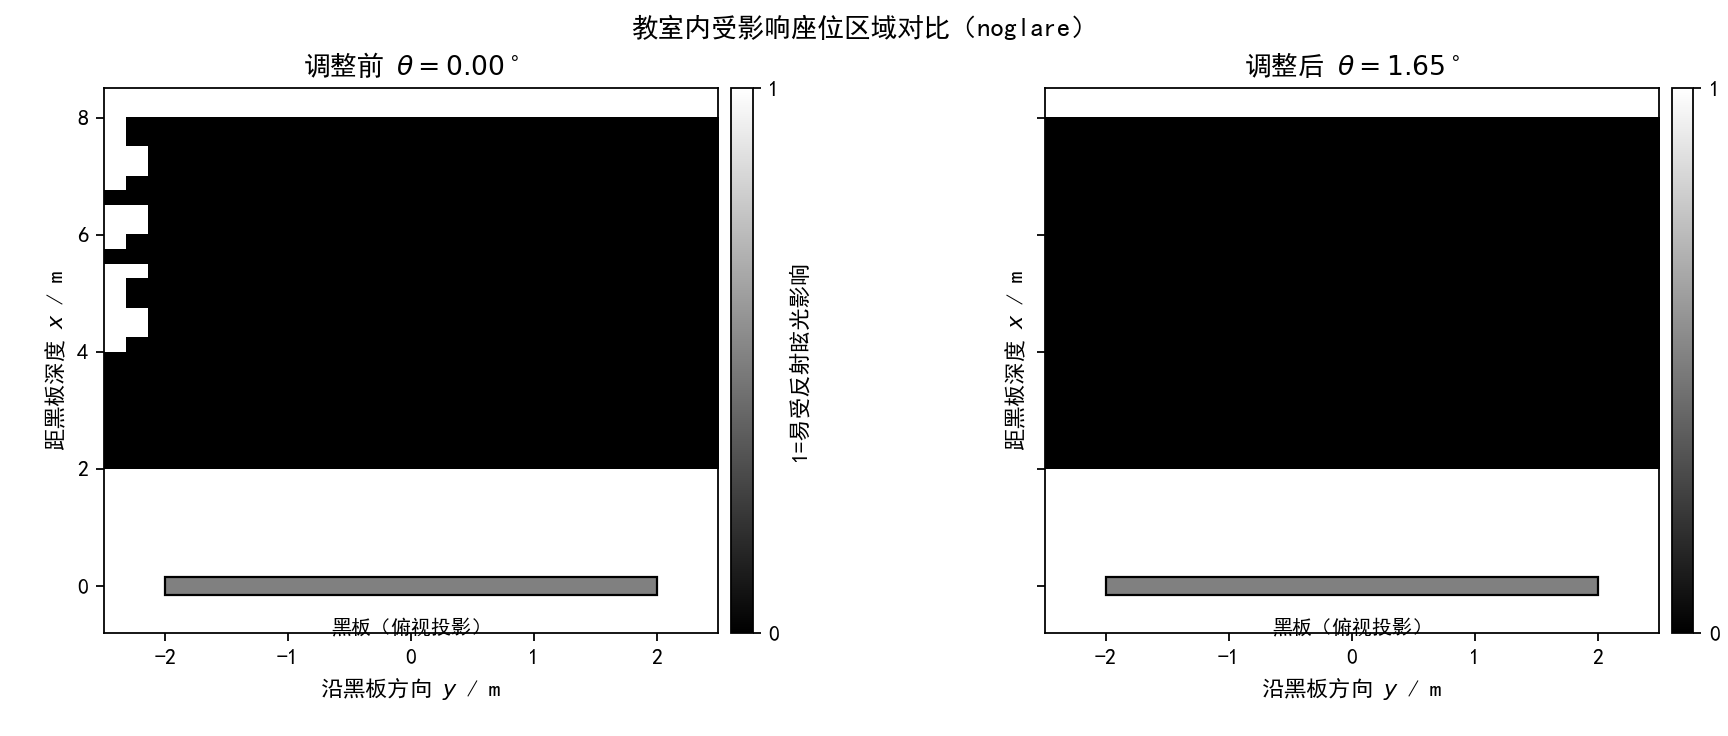
\includegraphics[width=\linewidth]{figures/topdown_compare_noglare.png}
  \caption{No-glare 时刻（$t=9{:}30$，$\theta=1.65^\circ$）：调节前局部座位受影响，调节后受影响格点为 0}
  \label{fig:topnog}
\end{figure}

\subsection{竖直截面光路示意}
图 \ref{fig:sec} 给出最坏示意时刻下，调节前后入射方向、法向与反射方向在 $xz$ 截面内的关系。为增强可读性，右图采用 no-glare 策略对应角度，并在图内直接标注“反射光与视线夹角”，便于直观看到调节后的偏离效果。

\begin{figure}[htbp]
  \centering
  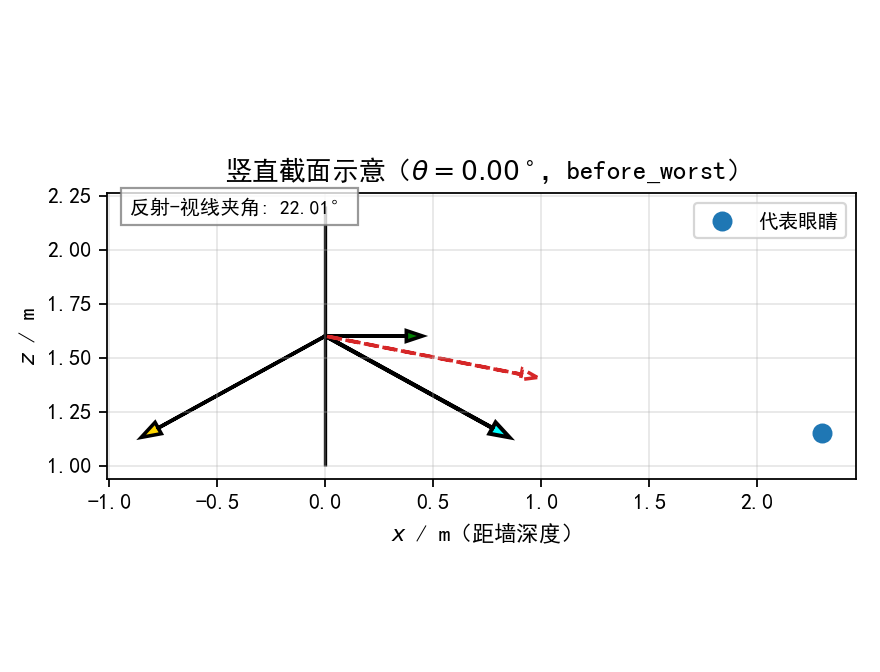
\includegraphics[width=0.45\linewidth]{figures/section_before_worst.png}\quad
  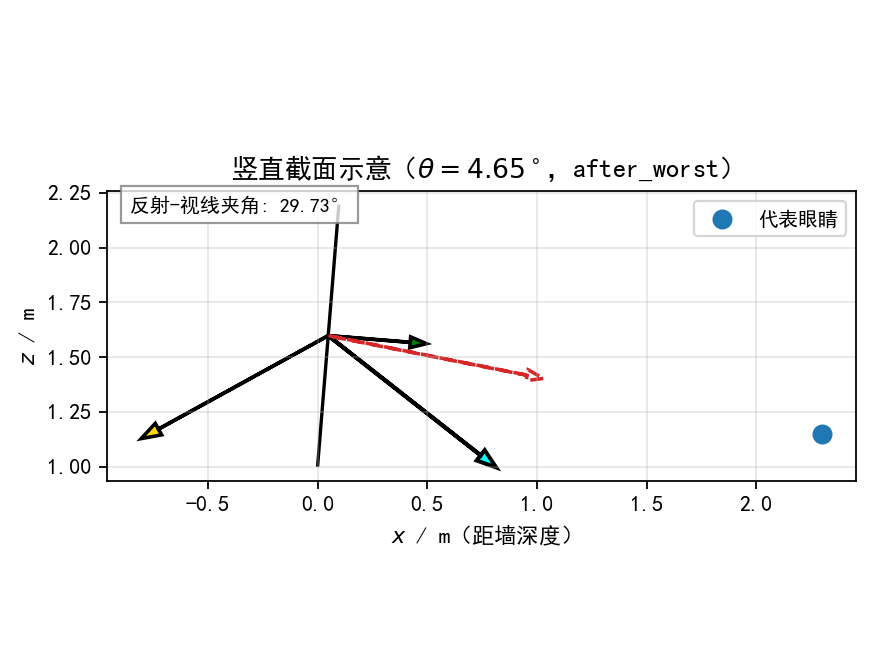
\includegraphics[width=0.45\linewidth]{figures/section_after_worst.png}
  \caption{竖直截面光路示意：调节前（左）与 no-glare 策略调节后（右）}
  \label{fig:sec}
\end{figure}

\section{灵敏度分析}
$\theta^\ast$ 与受害比例对以下因素敏感：阈值 $\varepsilon$、$\theta_{\max}$、窗户朝向与教室朝向组合、眼高 $h_e$、第一排距墙距离。提高 $\varepsilon$ 会扩大「受害」判定（更保守）；增大 $\theta_{\max}$ 可扩大可行域，但削弱书写舒适性约束的实际意义。

\section{改造方案（可落地）}
\begin{itemize}
  \item \textbf{结构：}黑板（或推拉绿板整体）下沿安装\textbf{可调铰链}，上沿或背部设\textbf{限位拉杆}，标定 $0^\circ$--$\theta_{\max}$ 刻度（建议 $\theta_{\max}\in[3^\circ,8^\circ]$ 由校方与厂商共定）。
  \item \textbf{使用规程：}早读、上午侧窗强光时段按示意图或简易日照表微调；平时回零。
  \item \textbf{协同：}极端角度仍不足时，优先\textbf{百叶/半帘}削弱平行光而非全遮光。
\end{itemize}

\section{模型评价}
\textbf{优点：}几何清晰，易于程序实现与可视化；「最小必要角」贴合教学场景。\\
\textbf{局限：}平行光与统一眼高为近似；未单独拆分一体机贴膜与粉笔板漫反射差异。\\
\textbf{推广：}可加入多扇窗离散光源、多排不同眼高、或目标改为「最小化受害座位数」的加权优化。

\section*{参考文献}
\begin{enumerate}
  \item 中华人民共和国住房和城乡建设部. GB 50033—2013 建筑采光设计标准[S]. 北京: 中国建筑工业出版社, 2013.
\end{enumerate}

\end{document}
